\documentclass{article}
\usepackage{spconf,amsmath,graphicx, cite, float, url}

% Example definitions.
% --------------------
\def\x{{\mathbf x}}
\def\L{{\cal L}}

% Title.
% ------
\title{Computer Security Report}
%
% Single address.
% ---------------
\name{Junsong Yang}
\address{School of Computer Science \\ University of Nottingham}
%
% For example:
% ------------
%\address{School\\
%	Department\\
%	Address}
%
% Two addresses (uncomment and modify for two-address case).
% ----------------------------------------------------------
%\twoauthors
%  {A. Author-one, B. Author-two\sthanks{Thanks to XYZ agency for funding.}}
%	{School A-B\\
%	Department A-B\\
%	Address A-B}
%  {C. Author-three, D. Author-four\sthanks{The fourth author performed the work
%	while at ...}}
%	{School C-D\\
%	Department C-D\\
%	Address C-D}
%
\begin{document}
%\ninept
%
\maketitle
%

\section{Passwords}
\label{sec:passwd}
In this section, the designed password and authentication policy will be proposed and justified.
First, the password policy will be explained in detail with additional authentication measures.
Then, mechanisms of storing passwords will be entailed.

\subsection{Password Policy}
As Gollmann \cite{GollmannDieter2011Cs/D}suggested, the overall security may be diminished 
if one security mechanism is overstated. Users tend to bypass the mechanism if it is too 
inappropriate for them to properly work with, hence the overall security of the system 
may be weakened. By considering that, the following password policies are proposed.

\subsubsection{Password Length}
This policy enforces the minimum number of character required to use as a valid password. 
Generally, the short the password, the more like and easily to be cracked by brute-forcing.
Hence, by setting the minimum password length to ten, the difficulty for brute-forcing password 
cracking would be noticeably increased.

\subsubsection{Password Format}
This policy intended to accumulating the strength of valid password by requiring what kind 
of character must be included in a password. By requiring the password to contain 
at least one lower and upper letter, one number, and one special character, combining with 
password length policy, the possibility of successful brute-force cracking would 
be significantly decreasing.

\subsubsection{Password Ageing}
This policy requires users to change their password periodically. The likelihood of password 
breaching would increase as time goes by, hence this is a appropriate approach to eliminate the 
risk of potential breaching.

\subsubsection{Password Use}
To further diminishing the risk of potential password breaching over time, additional mechanism 
need to be employed to block users from using the same password twice. This policy is essential 
to assist the password ageing policy to fulfil its purpose.

\subsubsection{Password Choice}
Dictionary attack is another approach frequently used for password cracking. The purpose of 
this policy is to prevent this attack. This problem can be addressed by preventing user from 
using the password in public known dictionary.

\subsubsection{Login Attempts}
This policy is designed to reduce the risk of brute-force attack. By limiting maximum number of 
failed login attempts the success rate of brute-force attack can be reduced significantly.

\subsection{Additional Authentication Measures}
Mechanism must be implemented to address the repeated authentication problem. 
Between time of check to time of use, user identity exploitation may occur as the 
authentication system does not keep track of what happened in between. 
Therefore, before some important actions like change password can be successfully performed, 
the user's identity need to be checked again to ensure the action is legitimate.

\subsection{Storing Passwords}
As suggested by Gollmann, password may be cached by browser\cite{GollmannDieter2011Cs/D}. Which 
suggests that storing raw password directly in database is a bad practice. To maximise security, 
password should be hashed using one-way hash function with salting and stretching approaches\cite{FergusonNiels2010Ce:d}.
Since hashing cannot be reversed, the original password will remain hidden.

\section{Firewalls}
\label{sec:firewalls}

%%%%%%%%%%%%%%%%%%% NOTES %%%%%%%%%%%%%%%%%%%%%%%%

% explain SSH tunnelling(VPN) which circumventing firewall restrictions
% example of legitimate use
% example of disreputable use

%%%%%%%%%%%%%%%%%%% NOTES %%%%%%%%%%%%%%%%%%%%%%%%
Firewalls are software or hardware that located between networks and filter potentially malicious 
packets from in and out traffic\cite{AndersonRoss1956-2008Se:a}.
Figure \ref{firewall} illustrates a network firewall which often stand between local system and 
the internet compare to the host-based firewalls which located on individual machines. 
According to Gollmann, firewalls can also prevent unauthorised accesses of the internal-only services which 
block unnecessary or potentially dangerous access of external services from inside of the network\cite{GollmannDieter2011Cs/D}.

\begin{figure}[H]
  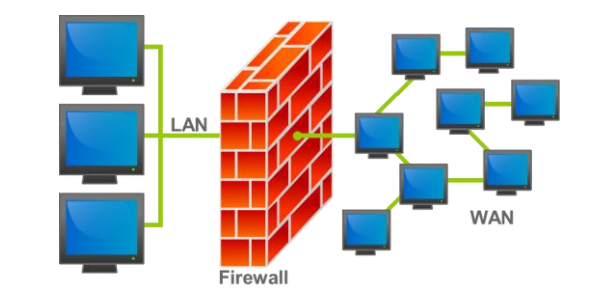
\includegraphics[width=8.5cm]{firewall}
  \caption{Network Firewall}
  \label{firewall}
\end{figure}

There several reasons that administrators may block port from normal traffic. As mentioned above, some services 
are only intended for internal access which suggests the necessity of blocking external access that 
may lead to security breaches. Another reason is that access external network from inside is also a potential 
breach in terms of the internal network as those ports are entrances to the network. 

As for internal network, some internal traffic is unnecessary even potential harmful. A peer-to-peer 
communication protocol BitTorrent, in this case, is most likely been blocked in some internal network.

\begin{figure}[H]
  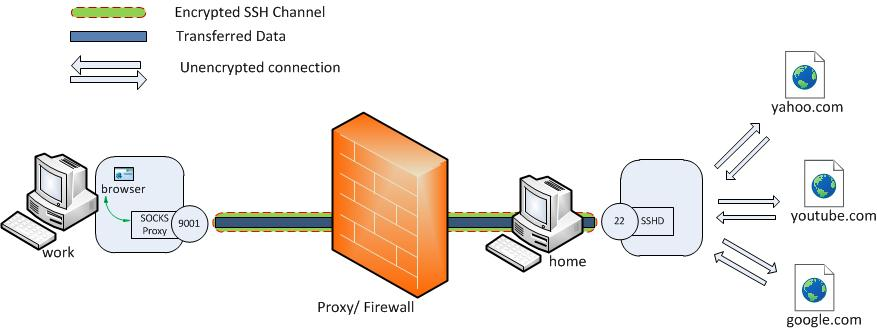
\includegraphics[width=8.5cm]{ssh}
  \caption{SSH Tunnelling}
  \label{ssh}
\end{figure}

Although some normal traffic is blocked or certain access rules are enforced by firewalls, there are ways 
to circumventing those rules and SSH tunnelling is one of them. 
SSH tunnelling is a way to establish encrypted communication channel between two computers. In terms of 
bypassing the firewall rules, SSH tunnelling serves as proxy. Figure \ref{proxy} shows how the proxy works 
in general. Since the target server cannot be accessed directly, the request is first sent to the proxy 
server in the middle. Then the proxy server forward the request to the target and return the response 
back the the client.

\begin{figure}[H]
  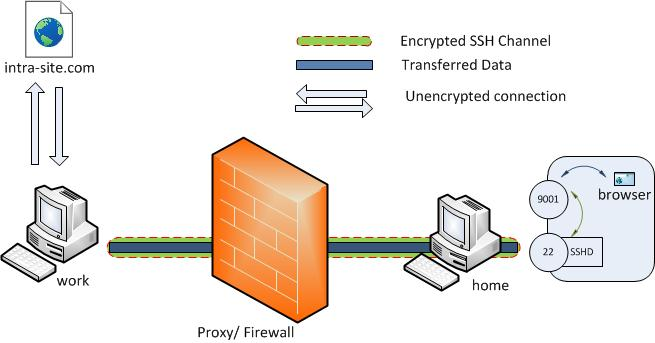
\includegraphics[width=8.5cm]{ssh1}
  \caption{(a) SSH Tunnelling\cite{chamith_2012}}
  \label{ssh1}
\end{figure}

Some usages of SSH tunnelling can be legitimate. As figure \ref{ssh1} demonstrates, the intra-site.com is 
a service only available from internal network. By establishing SSH tunnel with a machine inside the internal 
network, the internal services can be accessed from external. In this case, working remotely can be achieved. 
In fact, this approach is employed by most enterprises.

\begin{figure}[H]
  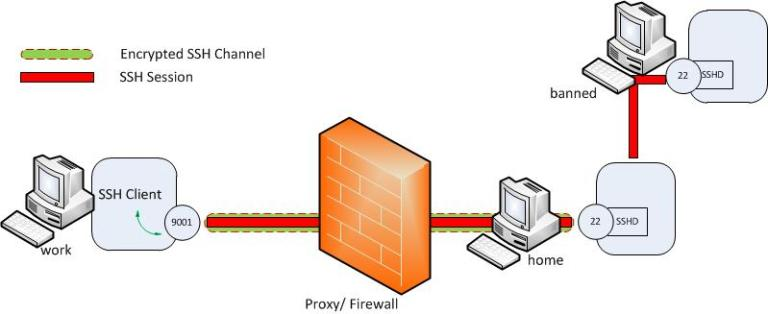
\includegraphics[width=8.5cm]{ssh2}
  \caption{(b) SSH Tunnelling \cite{chamith_2012}}
  \label{ssh2}
\end{figure}
Some usages of SSH tunnelling are disgraceful. In contrast to the example mentioned earlier, 
accessing blocked websites or services from internal network, as figure \ref{ssh2}demonstrates, 
exposes the internal network to the whole Internet. 
In this case, the internal is exposed under risks that the firewall built to eliminate which directly 
invalidated the firewall. Hence, this way of using ssh tunnelling is considered disreputable. 

\section{Server Security}
\label{sec:serversec}

%%%%%%%%%%%%%%%%%%% NOTES %%%%%%%%%%%%%%%%%%%%%%%%

%%%%%%%%%%%%%%%%%%% NOTES %%%%%%%%%%%%%%%%%%%%%%%%


% Below is an example of how to insert images. Delete the ``\vspace'' line,
% uncomment the preceding line ``\centerline...'' and replace ``imageX.ps''
% with a suitable PostScript file name.
% -------------------------------------------------------------------------



% To start a new column (but not a new page) and help balance the last-page
% column length use \vfill\pagebreak.
% -------------------------------------------------------------------------
%\vfill
%\pagebreak

\bibliographystyle{IEEEbib}
\bibliography{bibtex}

\end{document}
